% --------------- 12 POINT FONT -------------------------------
\documentclass[tog]{acmsiggraph}

% --------------- 10 POINT FONT FOR CAPTIONS ------------------

\usepackage{listings}
\usepackage[dvipsnames]{xcolor}
%%% Make the ``BibTeX'' word pretty...

\def\BibTeX{{\rm B\kern-.05em{\sc i\kern-.025em b}\kern-.08em
    T\kern-.1667em\lower.7ex\hbox{E}\kern-.125emX}}

%%% Used by the ``review'' variation; the online ID will be printed on
%%% every page of the content.

\TOGonlineid{45678}

%%% Used by the ``preprint'' variation.

\TOGvolume{0}
\TOGnumber{0}

% --------------- MATH PACKAGES -------------------------------
\usepackage{amsmath,amsthm,amssymb}

% -- Packages Added by Suhail
\usepackage{graphicx,epstopdf,subfigure,url}
\usepackage{listings}
\lstset{basicstyle=\ttfamily\footnotesize,
    frame=single,
    breaklines=true
}

\title{Processing collections of images and videos on big-data frameworks}
\author{Alex Poms, Ravi Teja Mullapudi, \\Suhail Rehman}
\pdfauthor{Alex Poms, Ravi Teja Mullapudi, \\Suhail Rehman}

\begin{document}


\maketitle

\begin{abstract}
\end{abstract}

% --------------- CONTENT -------------------------------------
\section{Introduction}
Images and video already dominate internet traffic and occupy a significant
amount of datacenter storage. The Cisco Visual Networking Index predicts that
IP video traffic will consume over 80\% of total internet bandwidth in 2019. In
2009, Facebook reported 1.5PB of image storage with 25TB added weekly and
550,000 images served per second at peak. This visual data is mostly just
served directly to a human user for viewing. However, recent advances in
computer vision, such as feasible image/object understanding and reconstruction
of 3D structure from image collections, motivate large-scale analysis of images
and videos for deriving insights and information that is not accessible from
other sources. For example, a relief organization could automatically
reconstruct the damage done by a natural disaster by having vehicles with
mounted cameras observe the affected area or a state could perform automatic
demographics estimation by analyzing the public Facebook profile photos of
their residents.

Currently, visual computing applications are few and far between due to the
inherent complexities of working with large visual datasets. The most apparent
of these difficulties is that the massive size of the datasets vastly exceed
the storage and computational capacity of a single machine. Thus any
application must be distributed and parallelized across a large cluster,
managing data transfer and communication between nodes. Unlike traditional
analytics workloads, visual computing applications also require highly tuned
and efficient image processing kernels that take advantage of the heterogeneous
hardware increasingly seen in cloud infrastructure, such as throughput-oriented
accelerators including GPUs and even FPGAs. Having a predefined set of
optimized implementations is not enough because image processing pipelines
require global code restructuring that crosses function boundaries; each
application may require custom image processing code that is composed with
other functionality. Lastly, visual computing applications exhibit tight
coupling between traditional analytics operations, such as those of Spark
\cite{zaharia2012resilient} and MapReduce \cite{dean2008mapreduce}, and
non-streaming operations, like distributed optimization or graph processing.

It is unclear if existing systems can simultaneously satisfy these three
requirements. Systems optimized for analytics operations, like Spark, tend to
sacrifice explicit access to their data collections that prohibit efficient
integration of non-streaming operations. Analytics systems also lack the
ability to specialize user routines to heterogeneous hardware resources. On the
other hand, systems that perform non-streaming operations, like the Parameter
Server \cite{li2014scaling}, generally lack the flexibility in their
programming model to allow direct incorporation of streaming operations like
map, filter, or reduce.

\section{Background and Related Work}

\subsection{Spark}
Spark \cite{zaharia2012resilient} is a large-scale data processing framework
for operating on distributed collections. Spark derives much of its design from
MapReduce \cite{dean2008mapreduce} but extends the abstractions provided by
MapReduce in two key ways: (1) composition of operations to into a lazy series
of operations and (2) in-memory fault-tolerance by allowing lost partitions to
be recomputed based on tracking the lazy series of operations (which they call
a \textit{lineage}).

% Spark Programming Model
A Spark user constructs a program by specifying a series of
\textit{transformation} operations on immutable distributed collections (called
\textit{RDDs}) that source their data from some stable storage (such as
HDFS). Spark does not perform any of these transformations until an
\textit{action} has been specified. Actions are operations which write data out
to a stable storage system or return results back to the user's driver
program.

% Spark Implementation

Conceptually, Spark programs are split into two types of stages. The first type
of stage, called a Result Stage, consists of series of point-wise
operations (such as map, filter, flatmap, etc.). The second type of stage,
called a Shuffle Stage, is composed of mapper nodes which write key
value pairs to local partitions followed by reducer nodes which fetch those
partitions based upon an assigned key and perform some a reduction operation on
all values belonging to a single key. The Shuffle Stage is exactly equivalent
to the Map and Reduce phases provided by the MapReduce programming model except
that partitions need not be written to disk before being collected by
reducers. The Result Stage does not have a direct parallel to anything in
MapReduce but is key to enabling the lazy programming model that Spark provides
to users. Spark implements a Result Stage by \textit{fusing} point-wise
operations together such that for each element in the input, Spark will execute
all transformations on that individual element before operating on any other
elements in the collection. Fusion is used by Spark to minimize the working set
size and thus support out-of-core collections efficiently but also has the side
benefit of optimizing for \textit{locality} because values are utilized
immediately after they are computed.

% Spark issues

\subsection{Legion}

\subsection{SciDB}
SciDB\cite{stonebraker2013scidb} is a computational array DBMS designed to
cater to the data storage needs of the scientific community. SciDB is designed
to be multi-dimensional, with an array-based data model. It also provides
support for data versioning and provenance which is a oft-cited feature
requirement of data management systems from scientists.

SciDB arrays are expressed in terms of two basic parameters: the {\em
dimensions} of the array, as well as {\em attributes} of the array.

An n-dimensional SciDB array has dimensions ($d_{1}$,
$d_{2}$,$...$,$d_{n}$). The {\em size} of each dimension is the number of
ordered values in that dimension. For example, a 2-dimensional array may have
dimensions $i$ and $j$, each with values $(1, 2, 3, ..., 10)$ and $(1, 2, ...,
30)$ respectively. SciDB uses 64-bit integers to represent the values in each
dimension, but also support non-integer dimensions such as variable-length
strings or floating point integers. Furthermore, SciDB supports the notion of
dimensional bounds. When the total value of a dimension is known in advance,
the array can be declared with a {\em bounded} dimension. Sometimes, the
cardinality of the array may not be known at array creation time. In such
cases, the array can be declared with an {\em unbounded} dimension. It must be
noted, however, that certain array operations are restricted to arrays with
integer bounded dimensions.

In addition to the dimension size attributes, the user must define two
parameters for each dimension: the {\em chunk size} and {\em chunk overlap}
parameters. These parameters affect the distribution of the array data among
the worker nodes and need to be studied with respect to their effect on the
performance of the image operations that we intend to deploy in SciDB.

An n dimensional array in SciDB refers to a single cell or element of an
array. However, each array in the SciDB array can hold multiple data values
known as {\em attributes}. Each data value is referred to as an {\em
attribute}, and can be any of the supported data types in SciDB.

Therefore, during the creation of an array in SciDB (analogous to the
declaration of a table schema in a relational database), the user must specify:

\begin{itemize}
\item An array name - a simple string which can be used to refer to the array
in all operations involving the array.
\item The dimensions of the array. The name and size of each dimension must be
declared, with the exception of unbounded dimensions, whose size is represented
using the asterisk character (\texttt{*}).
\item At least one attribute for the array. Attributes can be added to an array
as the result of an operation in SciDB.
\end{itemize}

An example of an array definition in SciDB is given below:

\begin{lstlisting}[caption=Creating an Array in SciDB, frame=single]
AQL \% CREATE ARRAY open <val:double>[I=0:9,10,0,J=0:*,10,0];
\end{lstlisting}

In the example, the name of the array is \texttt{open}, with one attribute
named \texttt{val}, of type \texttt{double}. This array consists of two
dimensions, \texttt{I} and \texttt{J}. \texttt{I} is a bounded dimension with
values ranging from 0 to 9, with chunk size 10 and chunk overlap 0. \texttt{J}
another dimension similar to \texttt{I}, but the size of this dimension is
unbounded.

SciDB is designed to perform a number of operations on Arrays. An extensive
listing of array operations is beyond the scope of this document, the
interested reader is referred to the SciDB manual\cite{SciDBManual}. However,
the operations that can be performed on an array can be broadly classified into
the following: array selection, array operations (such as cross product, joins
etc.), aggregation operations (which can return either arrays or scalars) and
so on.

\section{Workloads}
Visual data applications contain a diverse set of operations, but a few of them
stand out as particularly important and distinctly core components of the
analysis algorithms they are a part of. In particular, two classes
of operations that seem to span a significant amount of the space of important
operations in visual data applications are: very compute-intensive kernels
applied individually across an entire dataset, and aggregate,
high-communication operations, like computing nearest neighbors or
clustering. For a distributed computing framework to serve as a platform for
creating performant applications that process large collections of images and
videos, it must at least support very efficient and scalable implementations of
the following operations:

\subsection{High-performance map kernel}
An image is not simply an array of bytes. Images represent a set of
spatially-coherent samples over a regular grid. Processing an image into useful
information requires acknowledging this representation. Due to this essential
nature, algorithms which process images into information must perform
computationally expensive convolutions which operate over a spatial
extent. Convolutions exhibit high arithmetic intensity because the data
required to compute an output value highly overlaps with the data required to
compute neighboring output values. Thus after computing one value, the next
value already has most of the data required in cache and only needs to
perform the computation to compute itself.

Deep Convolutional Neural Networks (CNNs) have recently become a very effective
tools for extracting information from images. CNNs are trained for various
computer vision tasks like object classification, recognition and detection.
Networks which are used in these tasks are trained over massive datasets and
take weeks to train. However, networks trained for a task can be used to extract
features from an image which are useful for other computer vision tasks. CNNs
are organized as layers which successively process an input image. Features can
be extracted from an image by evaluating a trained network on input image and
taking the output of one of the layer. It is very common for a vision algorithm
to begin by evaluating a CNN on the entire dataset as the first step. This can
be viewed as mapping a CNN on the entire set of input images. The layers in CNN
especially the convolutions are very compute intensive and need highly optimized
implementations which utilize all the hardware resources.

\subsection{Clustering}

While analyzing a large collections of images, an operation that frequently
arises is finding similar images or discovering groups of images that are
similar. Both these operations involve computing distances between image
representations like feature vectors or even raw images themselves. Two
algorithms that are representative of aggregate operations on images are
k-nearest neighbors and k-means. The k-nearest neighbors algorithm finds the k
nearest neighbors to each item in the collection. An item in a collection could
be an image a or a feature vector representing the image. Similarly k-means
algorithm finds k representative items in the data set. Unlike map operations
which do not involve complex communication partitions, these operations need to
be decomposed carefully for controlling working set sizes and maintaining
locality.

\section{Distributed collections on Legion}

At a high level, research in high-performance distributed systems for data
analysis can be split into three camps. The first is the distributed systems
community, from which systems like Spark, MapReduce, and the Parameter Server
hail from. The areas of focus in this community that we see as having a large
impact on the big-data frameworks they have produced are fault-tolerance,
programming models that improve programmer productivity, and out-of-core
processing of data.

The second is the Supercomputing community, from which frameworks like MPI and
Legion \cite{bauer2012legion} originate. The values that the Supercomputing
community holds which are also important for visual data applications are
high-performance and compute-intensive tasks that fully utilize the machine,
regions which explicitly model data placement and layout, and complicated,
data-dependent task graphs.

The third is the Database community, of which systems like PostgreSQL and SciDB
are descendents of. Databases like SciDB hold out promise of a single system
that could support the complicated communication patterns of traditional
relational algebra operations, such as joins, with the high-performance
distributed processing required for computing on array-like data. However, as
seen in our evaluation, the performance is currently not up to the level
required of high-performance applications.

All three community's lines of research have produced research artifacts which
have properties that when combined could produce a system which is able to
efficiently and elegantly express many visual data applications. Our current
implementation of a distributed collections abstraction on top of Legion is a
first step toward taking some of the properties we have identified in the
disparate communities and trying to merge them together. We have chosen Legion
as a base framework because we believe that it provides a low-level layer on
which abstractions like the distributed collections provided by Spark can be
implemented using. It is not clear how using a system like SciDB or Spark as a
base would allow the system to provide the type of functionality that
the Supercomputing community's system provide.

\subsection{API}

Our system is built on top of Legion and thus is written in C++. The current
implementation is compiled as an static library that can be linked into an
application and is roughly 4500 lines of code. The user only needs to include
two header files (one that defines the context and one that defines the
collection operations) to start writing programs against it.

The current interface we provide can be roughly categorized into traditional,
data-parallel collection operations and aggregate, domain-specific
operations. The data-parallel operations are inspired by Spark and serve mainly
to provide a nice programming model that will increase programmer productivity.

\subsubsection{Data-parallel operations}
The current set of data-parallel operations provided are the following:

\begin{itemize}
\item \textbf{load} - loads an RDD from an implementation-defined storage.
\item \textbf{map} - applies a function to each element in a collection.
\item \textbf{filter} - returns all elements in a collection which fulfill a
predicate.
\item \textbf{flatmap} - linearizes all elements returned from applying a
  function to the collection that returns a list.
\item \textbf{reduce} - produces a single output value by successively combining
  elements using a function.
\item \textbf{collect} - materializes a collection in the user's driver program.
\item \textbf{save} - saves an RDD in implementation-defined storage.
\end{itemize}

These operations are exactly the same as provided by other data-parallel
systems except for the \textit{load} and \textit{save} operations. The load and
save operations provide a way for the system to automatically incorporate an
implementation-defined form of storage that can be optimized based on the type
of elements in a distributed collection. For example, if a collection contains
images or videos, the system can automatically infer that and compress the data
items using a perceptual compression format such as PNG or JPEG.

\subsubsection{Aggregate Domain-Specific operations}
Our system provides a set of specialized operators for the domain-specific
algorithms which can not be efficiently expressed using streaming
operations. The operations are:

\begin{itemize}
\item \textbf{K Nearest Neighbors} - given a collection of elements and a
  function for computing how similar two elements are to each other, returns a
  collection of the same size as the input where each element holds a list
  containing the K closest elements which matched to the element previously at
  the same position
\item \textbf{K Means} - for a collection of elements, typically vectors, which
  can be added together and averaged, returns K vectors which represent the
  ``mean'' vectors of the collection. This operations is performed by randomly
  initializing K cluster centers and successively iterating by find the closest
  points to each cluster center, averaging them together, and replacing the
  cluster center with that value. The algorithm converges when the cluster
  centers no longer move after being averaged.
\end{itemize}

The specific operations were chosen because they contain communication patterns
common to aggregate operations in many visual computing applications. While the
exact functionality they provide is somewhat limited, their implementation will
help reveal issues in achieving high-performance on these types of specialized
aggregate operations. The major outstanding question with regards to
domain-specific functions is whether the specialized operators will ultimately
be a set of highly optimized functions provided as built-in operations or if
there exists some common primitives which a significant portion of the
operators can be composed of. The second possibility is more attractive because
it means that the system could optimize composition of the routines and users
could easily extend the system with other algorithms. As papers like Halide
have shown, the composition of two highly optimized routines does not always
result in an optimal solution. Common primitives would mean that the system
could introspect dependent routines and co-schedule them for better
performance.

% impedance mismatch with fixed sized regions
%% Larger than memory
%% Dynamic amplification and decimation

\subsection{Task scheduling}

One of the most important advantages to implementing our distributed
collection abstraction on top of Legion is it allows us to easily schedule
operations on the underlying representation of the distributed collections
which contain complex and dynamic read and write dependencies. While it is
possible to implement a diverse set of aggregate operations on top of the
primitives provided by a system like Spark, it is not true that the most
efficient implementation can be efficiently expressed using those primitives.

\subsubsection{K Nearest Neighbors Implementation}

\begin{figure}
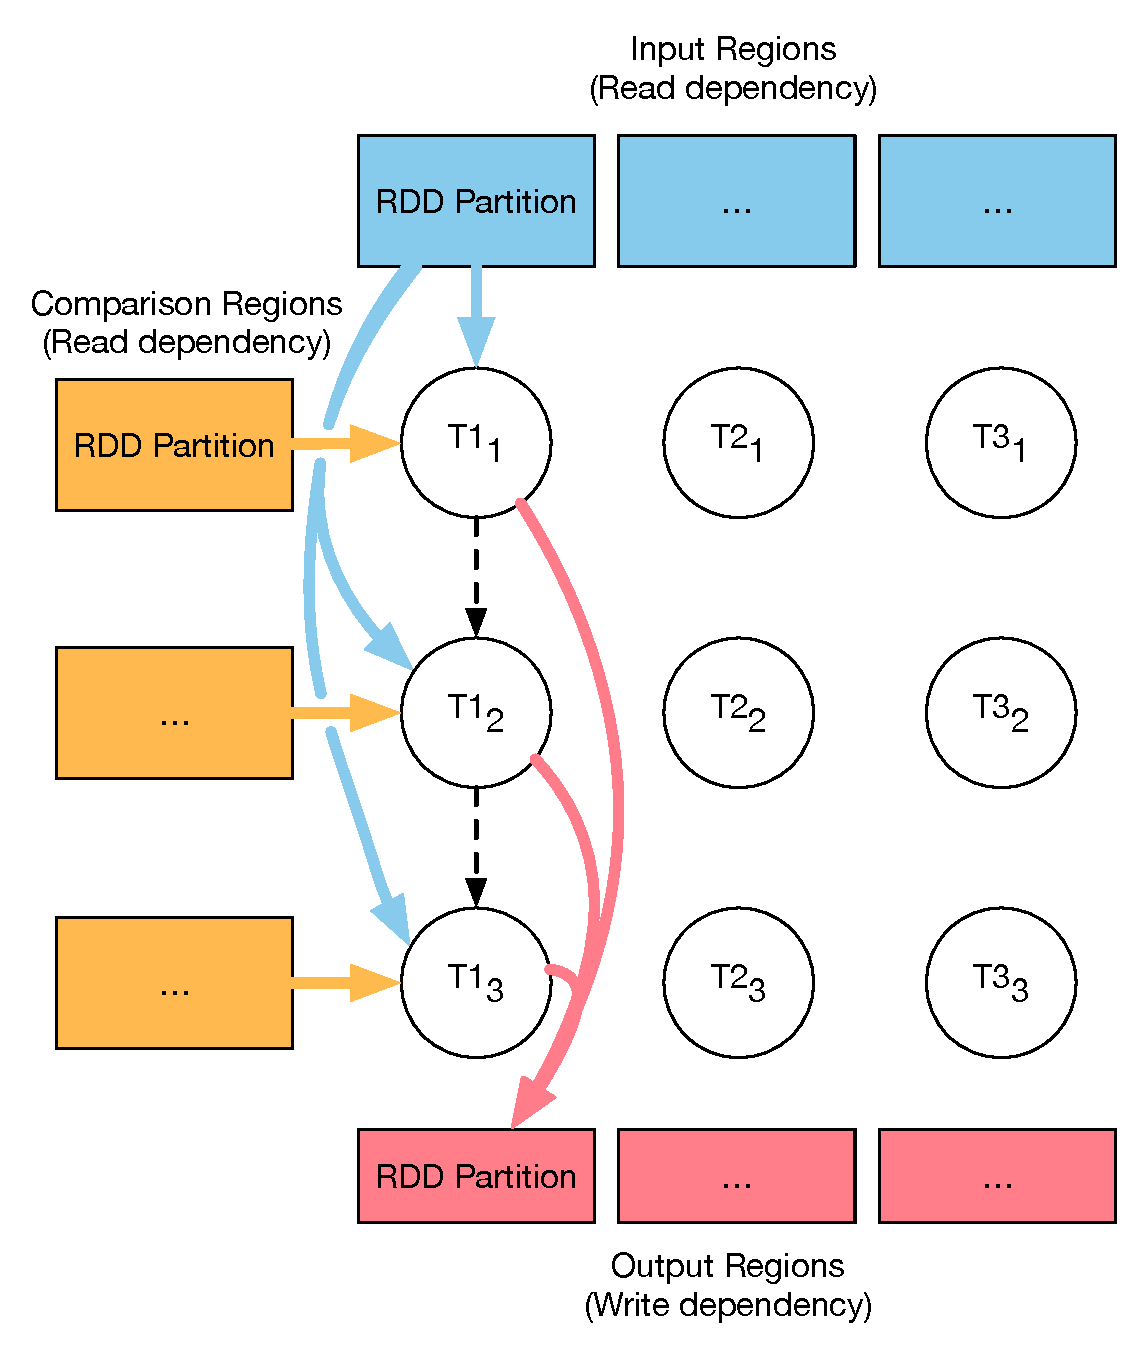
\includegraphics[width=0.45\textwidth]{figures/knn}
\caption{A K Nearest Neighbors implementation on top of Legion regions}
\label{fig:knn}
\end{figure}

To illustrate what the implementation of a domain-specific aggregate operation
looks like, we will briefly discuss our approach to K Nearest Neighbors. As you
can see in Figure \ref{fig:knn}, the input to K Nearest Neighbors is a single
collection of elements (seen in blue and orange) and the output is a collection
of lists of length K (seen in red). Instead of launching a task for every
pairwise element in the input collection or materializing all of them and
streaming over the pairs, we partition the input into fixed size chunks and
launch \(N^2\) tasks where \(N\) is the number of chunks. Each of these tasks
depends on a pair of chunks in the input as read dependencies (blue and orange)
and a single output chunk as a write dependency (red). The dotted black arrows
are implicit task dependencies determined automatically by Legion's dependence
analysis runtime.

\section{Evaluation}

The evaluation we performed is split into two distinct parts: one for directly
testing Spark against Legion, and another for testing SciDB vs MPI. We
separated our evaluation into these two parts because we observed early on that
the performance difference between SciDB and Spark/Legion was so many orders of
magnitude off that it did not seem fruitful to directly compare the two. That
said, it would have been nice to replicate the MPI implementations used to
compare against SciDB for the experiment we performed with Legion and Spark,
but time did not permit; we hope to explore this in future work.

\subsection{Spark vs Legion}

Cloud-based clusters are increasingly growing in popularity, especially for
small teams or individuals which are interested in running an analysis on data
but do not have the capital or need to purchase and administrate a large number
of machines. This type of use case is especially important for visual data
analysis because computer vision researchers, astrophysics or biologists, and
governmental organizations who wish to analyze their large collections of
images and videos are likely to fall into the aforementioned category.

\subsubsection{Experimental Setup}

Our evaluation of Spark and Legion was performed on Google Compute Engine, a
cloud Infrastructure-as-a-service product. Our dataset consists of 5151 images
stored on Google Cloud Storage that were extracted from several videos. For the
following experiment, we ran each test on a cluster of 20 Intel Ivy Bridge
nodes with 4 virtual CPUs (hyperthreads) and 15GB of memory. For Spark, we
launched a single executor per node using the YARN scheduling framework. For
our Legion framework, we ran one Legion task per node.

\subsubsection{High-performance Map Kernel}

\begin{figure}
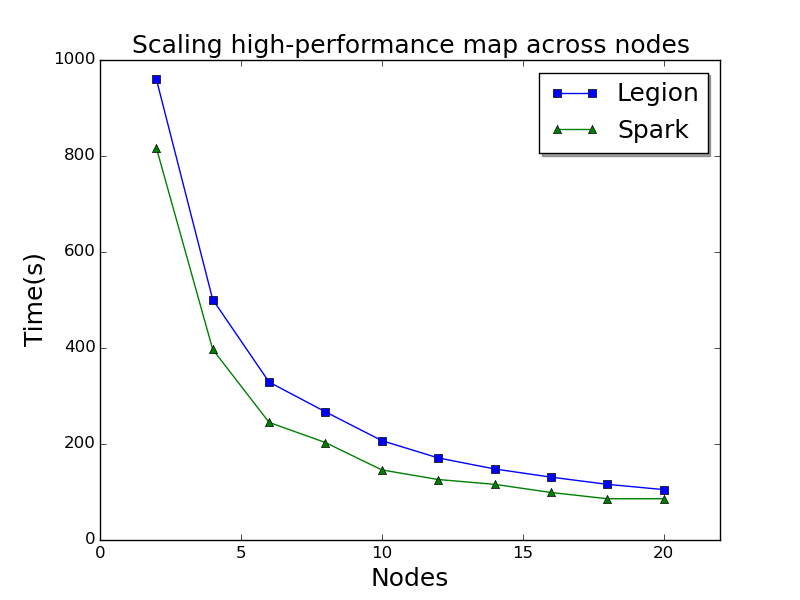
\includegraphics[width=0.45\textwidth]{figures/scaling}
\caption{Scaling of Spark and the Legion framework on a high-performance map
  kernel}
\label{fig:scaling}
\end{figure}

In this experiment, we loaded all 5151 images into a distributed collection in
both our Legion framework and in Spark and then compute a feature vector for
each image by mapping a neural network across every image. The MIT
Places-Hybrid network \cite{zhou2014learning} is our neural network of choice
because it is equivalent to the Krizkevsky et al. network topology
\cite{NIPS2012_4824} and has been used by modern visual data applications. This
is not the largest network that is used in the literature, but represents a
nice middle ground.

While both frameworks achieve very similar scaling, the Legion framework does
not exhibit the faster total runtime that we expected to see when running
against Spark. The primary discrepancy for the reduced performance in Figure
\ref{fig:scaling} for the Legion-based framework is due to our implementation
of the IO operations for retrieving data from Google Cloud Storage.

\subsubsection{Communication overhead}

To discover the exact source of unexpected performance numbers for the Legion
framework, we inserted timing calls into the implementation of the Spark load
and map operations and in our Legion framework load and map operations. For
each operation, we summed up all the time it took to compute each stage and
divided by the number of nodes.
\begin{center}
    \begin{tabular}{| l | l | l |}
    \hline
    & Spark & Legion \\ \hline
    Communication & 11.677 s, 13.44\% & 35.27 s, 32.28\% \\ \hline
    Computation & 75.181 s, 86.5\% & 73.9968 s, 67.72\% \\ \hline
    \end{tabular}
\end{center}
% Spark:
%% Communication: 11.677 seconds, 13.44%
%% Computation: 75.181 seconds, 86.5%
% Legion:
%% Communication: 35.2768 seconds, 32.28%
%% Computation: 73.9968 seconds, 67.72%

The issue is that in our implementation we wait for all of the communication to
be done for retrieving an image from Google Cloud Storage before performing any
other operations. This results in the total time taken per element to be the
sum of the communication and the computation performed. Spark does not suffer
this issue because they overlap communication and computation by pipelining
their communication operations. This is evidenced in the figure above where the
total time taken to perform the computation for our framework and Spark is
nearly identical but we spend a large fraction of time performing communication
because it is not batched together with multiple communication requests.

\subsubsection{Partition startup time}

\begin{figure*}[htp] \centering
\label{fig:scaling}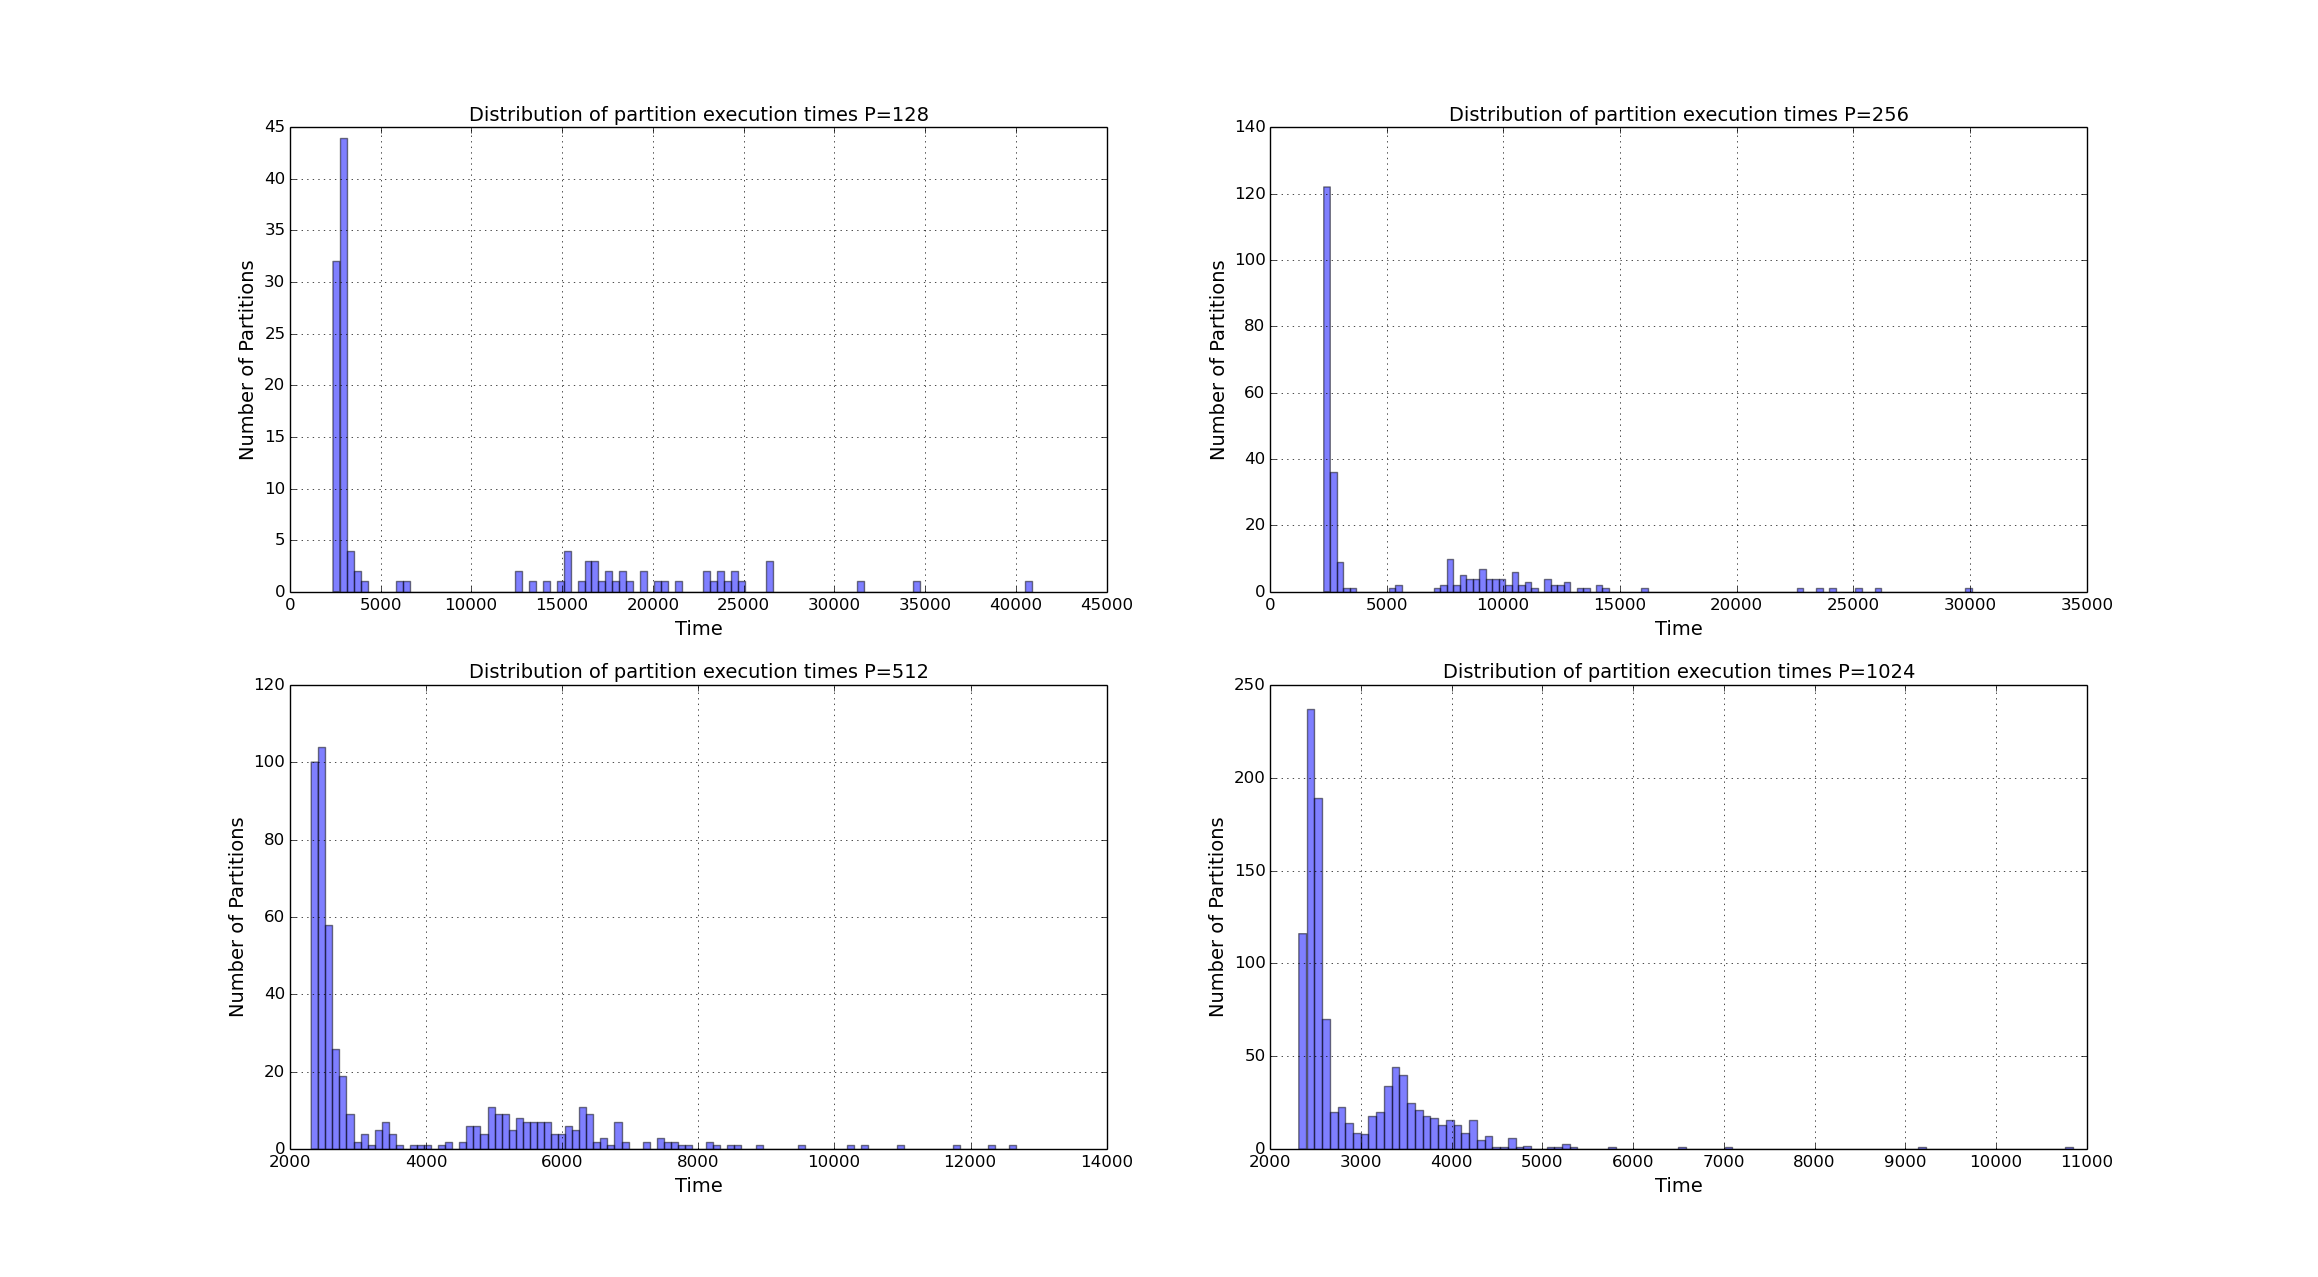
\includegraphics[width=\textwidth]{figures/partition_dist}
\caption{Distribution of task times for varying partition sizes on Spark}
\label{fig:partition}
\end{figure*}

In implementing the neural network in Spark, we had to utilize the
\textit{pipe} operator to execute the native code that ran the neural network
framework. Besides the increase in code complexity this introduces, having to
startup an external program and initialize a neural network for each partition
of the collection results in high overhead per partition and a minimum startup
cost. We measured this overhead by running the same experiment as before on 20
nodes with Spark but varying the number of partitions. As can be seen in Figure
\ref{fig:partition}, as we increase the number of partitions the number of
tasks which take around 2500ms increases. One strategy to alleviate load
balance from high variance in tasks is to introduce more partitions of your
dataset. The artificial startup cost we see here limits that ability because
smaller partitions are penalized by a minimum startup cost.

\subsection{SciDB vs MPI}\label{sec:clusterexp}
In this section, we compare the runtime of the image processing operations in
SciDB against their MPI counterparts.

\begin{figure*}[htp] \centering
\subfigure[WIA]{\label{fig:wia}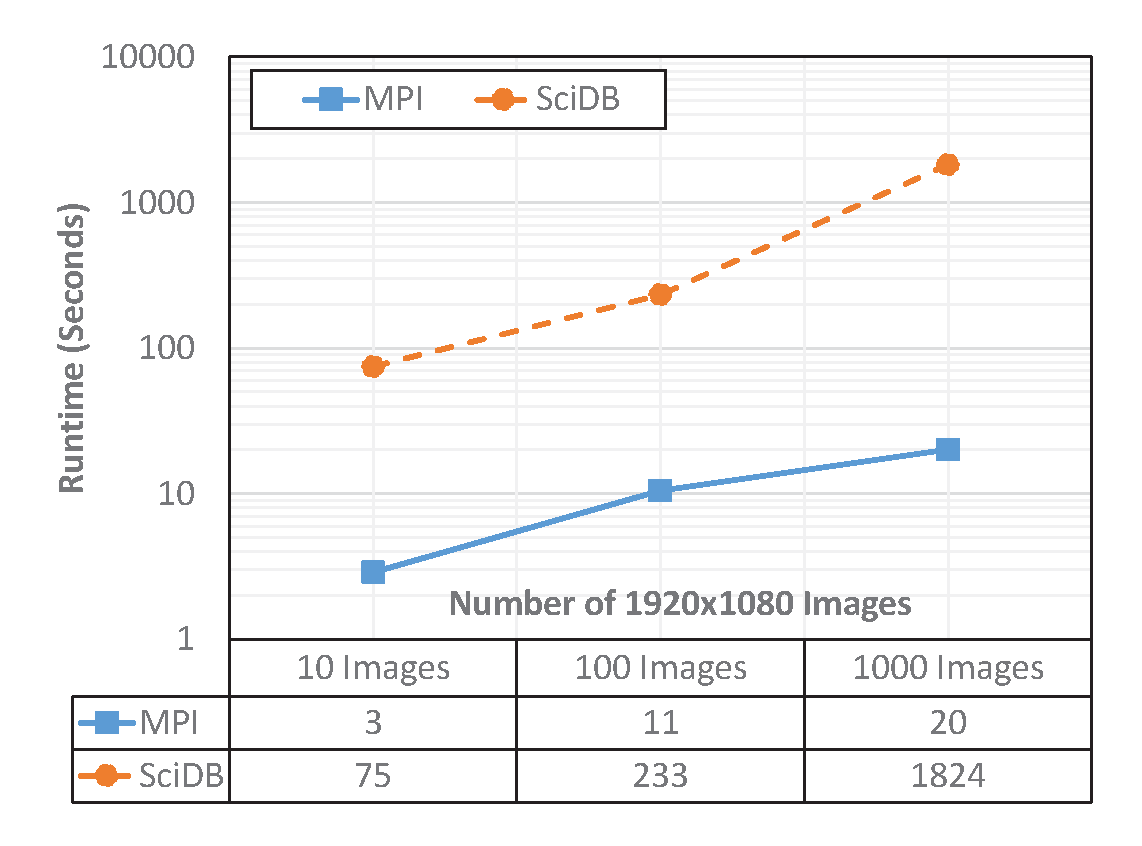
\includegraphics[width=0.45\textwidth]{figures/wia.eps}}
\hspace{1 em}
\subfigure[IPE]{\label{fig:ipe}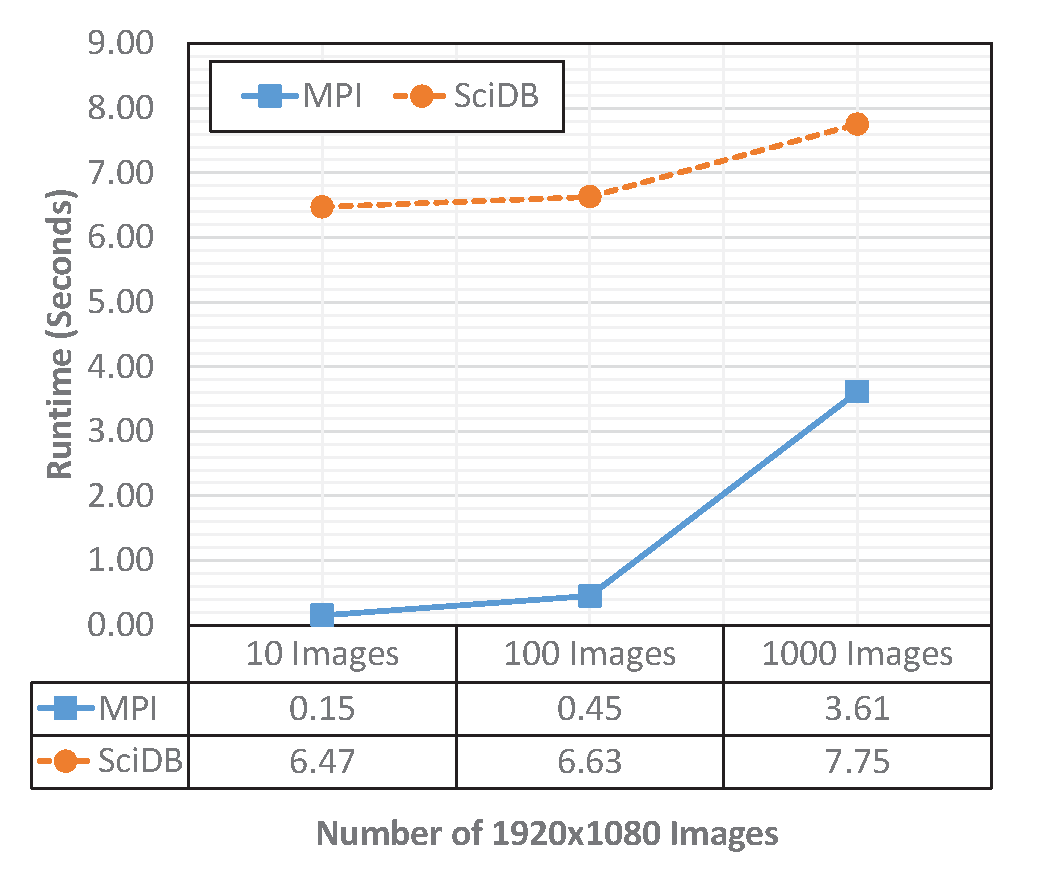
\includegraphics[width=0.4\textwidth]{figures/ipe.eps}}
\subfigure[CONV]{\label{fig:conv}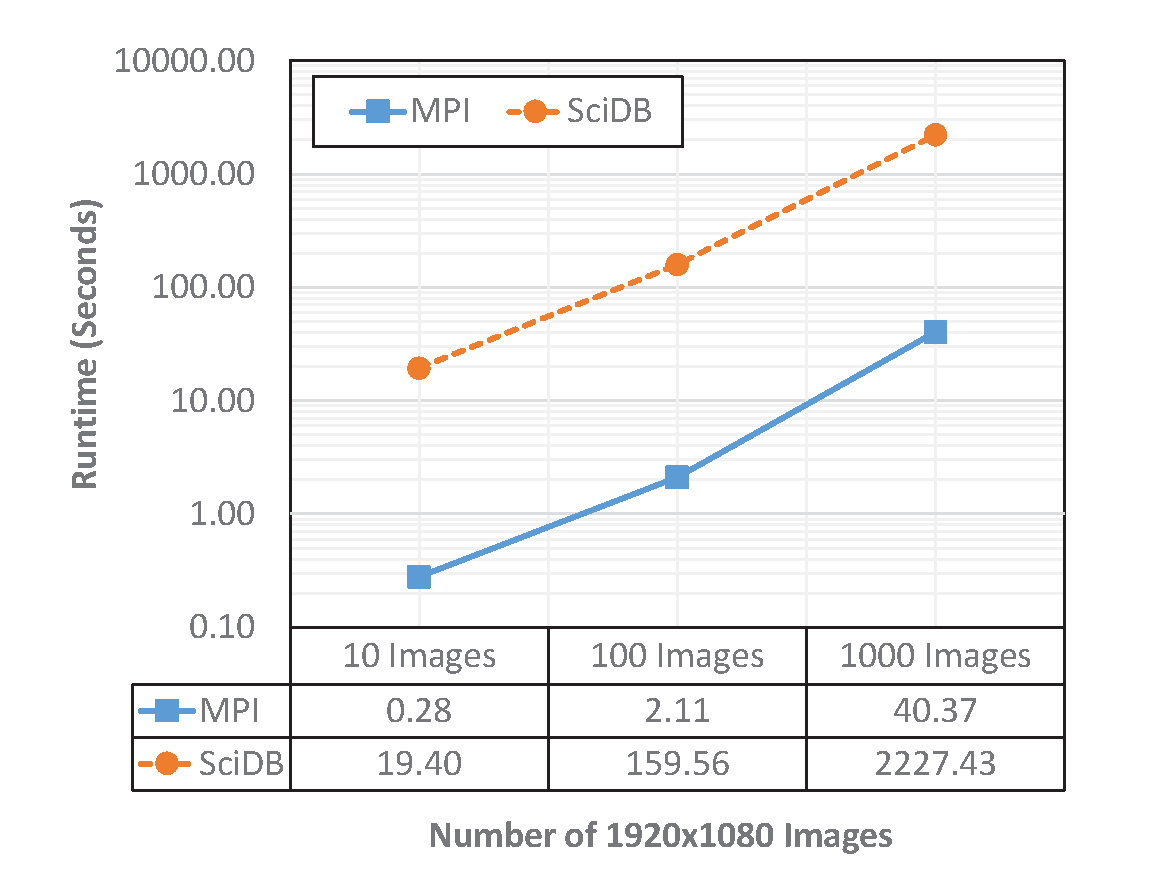
\includegraphics[width=0.5\textwidth]{figures/convo.eps}}
\hspace{1 em}
\subfigure[APNN]{\label{fig:apnn}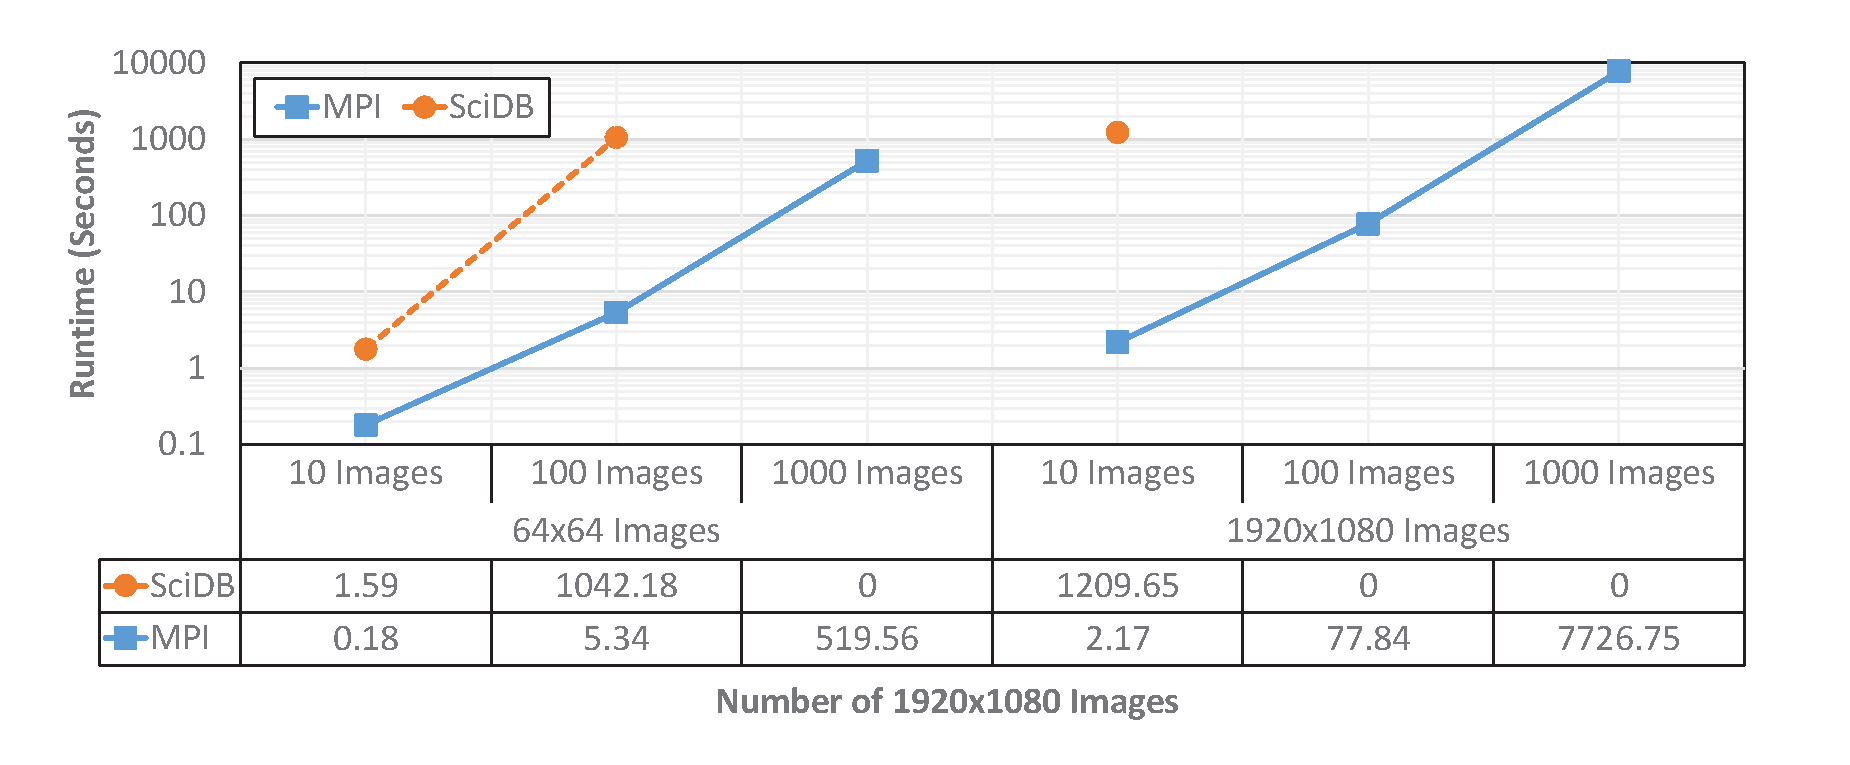
\includegraphics[width=0.85\textwidth]{figures/apnn.eps}}
	\caption{Performance of Image Operations in SciDB versus the Baseline MPI
Versions. All run-times are the average of 3 runs, with variation being within
\~2\% of the actual runtime. APNN benchmarks for larger datasets did not finish
running even after 6 hours.}
	\label{fig:mpi_result}
\end{figure*}

\textbf{Weighted Image Average}: In Figure \ref{fig:wia}, we see the runtime of
SciDB for the WIA benchmark for 10, 100 and 1000 images on the 16 node
cluster. The MPI version of this operation is roughly between $21\times$ to
$91\times$ faster than the SciDB counterpart for the same operation.

\textbf{Image Patch Extraction}: In Figure \ref{fig:ipe}, we see the runtime of
SciDB for the IPE benchmark (fixed patches) when varying the dataset
size. Unlike the WIA benchmark, where the entire image volume was flattened to
a single image, the IPE benchmark shows significant improvement in runtime and
is within an order of magnitude in terms of performance when compared to the
baseline MPI version, as the $100\times100$ image patch extraction and
averaging of a 1000 1080p images is only $\sim 2.14\times$ slower than its
corresponding MPI version.

\textbf{Convolution} In Figure \ref{fig:conv}, we compare the performance of
the MPI baseline that performs convolution on a set of images against the SciDB
\texttt{window()} function, which performs the equivalent operation. Again,
SciDB is an order of magnitude slower than the MPI implementation across the
board.

\textbf{All Pairs Nearest Neighbours}: For the APNN benchmark, we perform the
APNN step with an additional set of images: 10, 100 and 1000 64x64 thumbnails
(Figure \ref{fig:apnn}. The missing data-points indicate SciDB failing to
finish execution even after ~6 hours of runtime.


\subsubsection{Timing Breakdown and Analysis}\label{sec:breakdown} We now
provide the timing breakdown for two of the operations of interest, the WIA and
APNN benchmarks in Figure \ref{fig:breakdown}. We can see from the figures that
the runtime for these queries is dominated by the cross join query, more so for
APNN.

\begin{figure*}[htp] \centering
\subfigure[WIA]{\label{fig:wiabreak}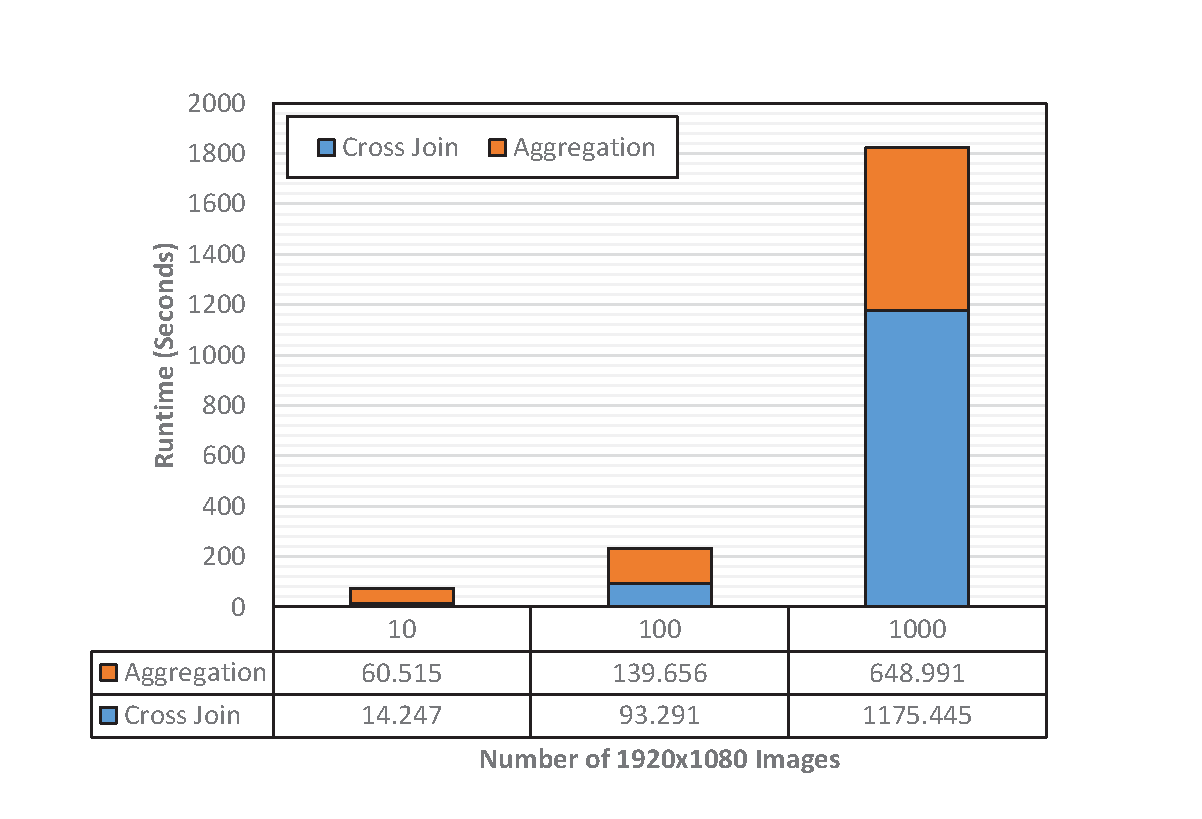
\includegraphics[width=0.50\textwidth]{figures/wia_breakdown.eps}}
\hspace{1 em}
\subfigure[APNN]{\label{fig:apnnbreak}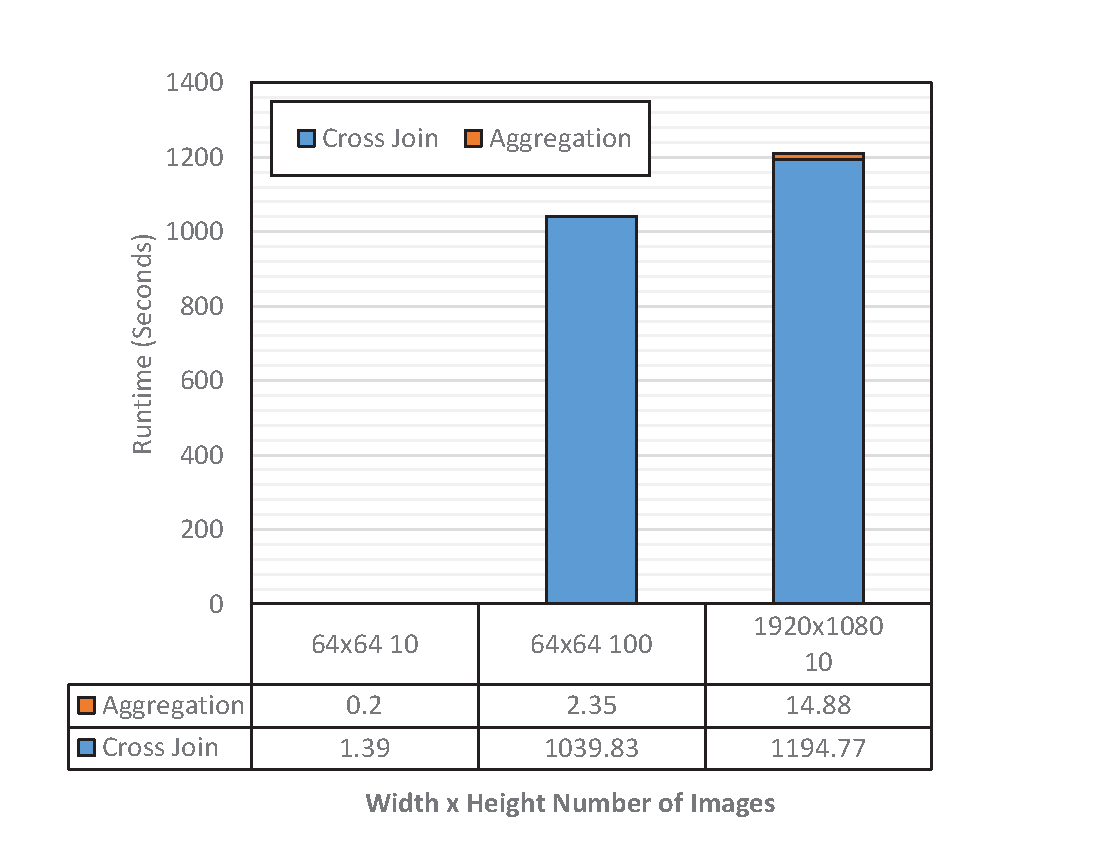
\includegraphics[width=0.45\textwidth]{figures/apnn_breakdown.eps}}
	\caption{Performance of Image Operations in SciDB versus the Baseline MPI
Versions. All run-times are the average of 3 runs, with variation being within
\~2\% of the actual runtime. APNN benchmarks for larger datasets did not finish
running even after 6 hours.}
	\label{fig:breakdown}
\end{figure*}

\section{Discussion and Conclusion}

\subsection{Improving SciDB}
SciDB is many orders of magnitude slower than the corresponding MPI
implementation and we conjecture the following reasons that contribute towards
the slow performance of SciDB:

\begin{itemize}
\item SciDB stores raw pixel values and is unable to take advantage of
domain-specific image compression schemes such as JPEG. This leads to a rapid
expansion of the number of images stored which, in turn leads to massive I/O
traffic during loading and execution of operations in SciDB.
\item Except for Convolution, all of the image processing operations studied
require some kind of cross-join operation, with APNN requiring a cross-join
across the image dimension, leading to massive increase in the amount of data
to be materialized.
\end{itemize}

The idea of SciDB or other array databases to perform image processing is
interesting as it allows for these operations to be expressed in the form of
queries. However, given the lack of support for domain-specific compression
formats and the extremely slow execution times, we believe there a lot of work
to do before SciDB becomes a viable platform for image and video processing.

\subsection{Merging two worlds}

From our experience in both frameworks namely Legion and Spark, we have
identified the characteristics of these systems that are beneficial for visual
computing workloads. We discuss the various design choices a future system needs
to address in the context of these characteristics.

\subsubsection{Mapping}
Mapping is the process of assigning partitions or tasks to each node. Legion
provides a default mapper which does a naive mapping that maximizes parallelism.
A Legion user is expected to make partitioning and mapping decisions based on
understanding of the application as well as the target cluster configuration.
Spark on the other hand only gives control of the partitioning and does the
scheduling automatically. Providing the ability to specify a mapping gives
flexibility and enables potential optimization. However, it is very cumbersome
for an user that is unaware of the target system and requires reasoning about
issues that are orthogonal to the algorithm. We believe that providing good
automatic mapping like Spark is one of the key ingredients going forward.

\subsubsection{Working set size}
Legion is primarily designed for applications whose working set fits in the
aggregate memory of all the systems in the distributed cluster. The
intermediates generated while working on large image collections can easily
exceed the aggregate memory of the cluster. Spark on the other hand is designed
with out-of-core data as a primary concern hence the support for backing
intermediates to disk and materializing them back from disk are
seamless. Bridging this gap requires adding support for disk backed regions in
Legion which is an avenue for further investigation.

\subsubsection{High-performance Kernels}
As we have discussed earlier a lot of visual computing operations are compute
intensive. Support for high-performance kernels implementing these operations is
very important in efficiently doing these operations. The Spark ecosystem is
tied to the Java Virtual Machine (JVM) which precludes utilizing many of the
high-performance kernels written in C++/CUDA natively. Getting around this
requires piping a Spark partition to an external process to  perform the
high performance kernel, as we done in the case of the high performance map.
This process is quite cumbersome and tedious since it requires stitching
together many systems. Legion is built in C++ and with heterogeneity as a first
class concern which enables integration with high performance kernels
seamlessly.

\subsubsection{Data allocation}
The size of regions in Legion is expected to be know at the time of allocation.
This is not an impediment to applications in which the number of items in a
collection is known upfront. For example, the number of points in a 3d-grid on
which a simulation is being run. However, this does not hold for processing
visual data like videos and images. Consider the case where each item in a
collection is a image and a flatMap operation which returns all the bounding
boxes of an object location in an image. One cannot know the dimensions of the
flatMap output region without computing the operation. Spark RDDs do not have
such restrictions and are completely defined at runtime.



\bibliographystyle{acmsiggraph}
\nocite{*}
\bibliography{final}

\end{document}
%%% Local Variables:
%%% mode: latex
%%% TeX-master: t
%%% End:
